%
%  index
%
%  Created by  on 2007-05-10.
%  Copyright (c) 2007 Texas Tech University. All rights reserved.
%
%\documentclass[twocolumn]{article}
\documentclass[12pt ]{article}
% Use utf-8 encoding for foreign characters
\usepackage[utf8]{inputenc}

% Setup for fullpage use
\usepackage{fullpage}

% Uncomment some of the following if you use the features
%
% Running Headers and footers
%\usepackage{fancyhdr}

% Multipart figures
%\usepackage{subfigure}

% More symbols
\usepackage{amsmath}
\usepackage{amssymb}
\usepackage{amsthm}
\usepackage{algorithm,algorithmic}
\usepackage{doublespace}
\usepackage{graphicx}
%\usepackage{latexsym}
\newtheorem{thm}{Theorem}[section]
\newtheorem{adef}[thm]{Definition}
\newtheorem{cor}[thm]{Corollary}
\newtheorem{lem}[thm]{Lemma}
%\theoremstyle{definition}


% Surround parts of graphics with box
\usepackage{boxedminipage}

% Package for including code in the document
\usepackage{listings}

% If you want to generate a toc for each chapter (use with book)
\usepackage{minitoc}

% This is now the recommended way for checking for PDFLaTeX:
%\usepackage{ifpdf}

%\newif\ifpdf
%\ifx\pdfoutput\undefined
%\pdffalse % we are not running PDFLaTeX
%\else
%\pdfoutput=1 % we are running PDFLaTeX
%\pdftrue
%\fi

\title{An Independent Component Analysis experiment using Distributed Computing Group Renaissance.}
\author{ Daniel Beatty }

\date{2007-05-10}

\begin{document}

\maketitle


\begin{abstract}
\end{abstract}

\section{Introduction}
The original assignment is 
\begin{quote}
	This project is to illustrate how a modified Independent Component Analysis (ICA) can be used to restore an image corrupted with additive Gaussian noise.  

	Choose any natural image (of a reasonable size), add 30\% Gaussian noise to the image, assuming a noisy image model:
	\begin{equation}
	\vec{z} = \vec{x} + \vec{n}
	\end{equation}
	%where include picture  \\
%	``http://www.cis.hut.fi/aapo/papers/IJCN99\_tutorial/img163.gif'', mergeFormatInet is Gaussian, and include picture \\ ``http://www.cis.hut.fi/aapo/papers/IJCNN99\_tutorialweb/img8.gif'' where mergeFormatInet is non-Gaussian.  
	
	Denoise the noisy image by using the Sparse Code Shrinkage Method (closely related to ICA) as described in the following in the following reference. 
	
	Compare the restored image using the above method with standard noise removal filters such the simple median filter or the Wiener filter. 
	
	MATLAB codes for various versions of ICA are available from the home page of A Hyv$\ddot{a}$rien and the Laboratory of Computer and Information Science at the University of Helsinki. 
\end{quote}

The best examples of MATLAB for this exercise is found in \cite[159-162]{stone-ica-tutorial}.  The versions of ICA included are gradient ascent, and projection pursuit.  %Descriptions of the ICA algorithm are best described in \cite{appo-ica-book} from chapter 7 to the end.   
ICA procedures determine both the mixing matrix and independent components from source data as shown in equation \ref{standardICA}.  
%One subject that should not be overlooked are the c
Contributing parts to each of the ICA algorithms include families of principal component analysis (PCA), entropy, estimators, and random variable properties.  This report illustrates the implementation of this family % families as 
frameworks for the Objective-C language.  At the time of this report, the version of Objective-C used is version 1.x.  %Also, the topic of Core Image versions were considered but not included in this report to allow for thorough research. 

There does exist another framework that could be used in Objective-C in the form of the IT++ libraries which are provided free under the GNU Public License.   The difference in the these two framework are as follows.  

First, the Distributed Computing Groups (DCG) version uses the Renaissance libraries as the basis for its matrix, and the IT++ uses a special version of matrix representation.   While there is nothing particularly wrong with either one, getting the data back out of DCG-Renaissance is much simpler as the data structure is a simple two dimensional double precision floating point which can be accessed directly.   

Second, the renaissance frameworks closely mirrors the proposed CI-Renaissance frameworks, which are a set of GPGPU equivalent frameworks that can take advantage of the graphics card hardware when available.   %Third, the 
Consequently the implementation of ICA in the DCG framework %is simpler allowing
 allows for one class per object for each type of ICA.  This allows the developer to use selectors to dynamically chose which ICA algorithm is desired.

%In the absence of MATLAB, this paper is resorting to using the implementation of the Fast ICA as implemented in the IT++ libraries provided free of charge under the GNU Public License.  Furthermore, this experiment uses a wrapper framework to IT++ called Cocoa IT build especially for this project.  

%The key to Sparse Code Shrinkage using ICA is in the summary provided in section 4 \cite[4]{hyvarinen99sparse}

%The specifications of Sparse Coding Shrinkage are satisfied as a product of the objects that satisfy ICA.  Independent components (ICs) are defined in terms of a fundamental equation, equation \ref{fundamental-ica}.  The observed data, $\vec{x}$, is result of a mixing matrix, $\mathbf{A}$, transforming a set of ICs, $\vec{s}$, plus some noise, $\vec{\nu}$.  ICA assumes that $\mathbf{A}$, $\vec{s}$, and $\vec{\nu}$ have no prior state.  ICA also renders $\vec{\nu}$ insignificant under the assumption that noise is normal.  There reasoning for this is explained with the notion of projection pursuit.   This report will show that satisfying $\mathbf{A}$ under the constraints of ICA also satisfies the mixing matrix for Sparse Coding Shrinkage.  

In order show that satisfaction of ICA objects ensures satisfaction of Sparse Coding Shrinkage% assertion of mutual satisfaction
, this report first examines the contributing frameworks of ICA, in section \ref{components}.   Section \ref{mutual-independence} shows the connection between the composing algorithms and and the many forms of ICA.   Section \ref{ica-scs-connection} shows the connection between ICA and Sparse Code Shrinkage. % Code, experiments, and results.


%Also in the first bullet, the probability density function is used specifically in non-polynomial versions of ICA.  Each version of ICA can be described in terms of how it achieves maximum entropy for each independent component.   These methods include entropy, mutual information, Kullback-Libler, maximum-entropy, negentropy, kurtosis, and non-polynomial negentropy.   Each of the entropy oriented methods work on the basis that non-normal is independent, and iteratively maximizes the non-normal component. 


%An experiment to demonstrate these equations simply takes an image, generates the $\mathbf{W}$ matrix. feeds in a noisy version of the same image into $g_i$.   This is done following the tutorials for Octave.    

%This same experiment is also done using Cocoa.  Admittedly, this implementation is far easier than the one for PCA.   One, no points of interest are being considered.  Thus the GUI for this exercise is much simpler.   Also, Core Image filters can be directly applied.   

%\newpage

\section{Families of Components}\label{components}

There is a concept learned from the Core Image model \cite{apple-core-image} that proves to be useful in these cases.  That is to design each of the components for ICA as specific purpose objects.  Each object consists just the necessary components necessary to construct the results for the object's purpose.  %, which are computed by the message apply.  % takes a set of arguments such as a matrix, a vector, a scalar or some state value.   The result can be defined with one word, ``apply.''   
Each object has a message apply which instructs the object to construct its results based on its existing members.  
As such, there is a family of components contributing to ICA, in addition to the specific purpose ICA objects themselves.   %Those families happen to be the chapters of \cite{appo-ica-book}, and listed here:
The frameworks containing these objects include:
\begin{itemize}
	\item Renaissance itself (DCGRenaissance)
	\item Random Vectors and Tests for Independence (DCGRandom)
	\item Estimators (DCGEstimators)
	\item Entropy (DCGEntropy) 
	\item Principle Component Analysis which is both part of DCGRenaissance and scheduled to expand into a new framework, DCGPrinciples.
\end{itemize}
In other literature, the specific purpose objects are called kernels.  To distinguish this paper from operating system literature, the term kernel here is reserved for Core Image kernels.  The family of components happen to be Objective-C frameworks.  
%Two things required for the ICA family are:
%\begin{itemize}
%	\item A good set of principal component analysis kernels
%	\item Good kernels for each form of ICA.
%\end{itemize}


\subsection{DCGRenaissance}

\subsubsection {DCGMatrix}
Consists of basic operations necessary a matrix in linear algebra.  Subsequent operations of linear algebra are designed to be separate and work on DCGMatrix.  A convenience  object named blasWork is used combine each operation objects in a MATLAB like scheme.  The operation objects such as add, subtract, and multiply so that the code for these operations is written and proven just once and therefore reducing error.   There are %combined 
also operation objects for vector-matrix interaction.  

\subsubsection{Gram-Schmidt Orthogonalization}
One significant operation object handles the Gram Schmidt Orthogonalization.  
%An example of classes designed to work on DCGMatrix is class named DCG-Gram Schmidt Orthogonalization (DCGGramSchmidt).   
Theorem \ref{gso-theorem} states that an vector space $\mathbf{V}$ can be transformed in to another vector space $\mathbf{W}$ such that each $\vec{w}\in \mathbf{W}$ is orthogonal.  Gram Schmidt Orthogonalization is a procedure based on theorem \ref{gso-theorem} that constructs each $\vec{w}_i \in \mathbf{W}$ on right after the other, and is defined in algorithm \ref{alg:gso}.
%As stated in theorem \ref{}, the goal of this class is to construct Gram Schmidt orthogonalization of a matrix consisting of column wise vectors.  The result is also a column wise matrix whose columns are orthogonal to one another.   

\begin{quote}
\begin{thm} 
\label{gso-theorem}
Suppose $w_1, w_2, ..., w_n$ form an orthogonal set of non-zero vector in $\mathbf{V}$.  Let $v$ be any vector s.t. $v \in \mathbf{V}$.  Define $v'$ s.t. 
\begin{eqnarray}
v' = v - c_1 w_1 - c_2 w_2 - ... - c_n w_n \\
c_i = \frac{\langle v , w_i \rangle} {||w_i||^2}
\end{eqnarray}
Then $v'$ is orthogonal to $w_1, w_2, ..., w_n$.
\end{thm} \cite[211]{schaums-linear-algebra}
\end{quote}


\begin{algorithm}
\caption{Gram Schmidt Orthogonalization}
\label{alg:gso}
\begin{algorithmic}
	\REQUIRE Column Wise Source Matrix: $\mathcal{V}$
	\STATE $N$ is the number of column vectors in $\mathcal{V}$
	\STATE Base case $\vec{v}_0 = \vec{w}_0$ 
	\STATE initialize $\vec{\theta}^0$, $T$, and $i \leftarrow 0$
	\STATE $v_0 \leftarrow $ [V columnVector:1]
	\STATE [W insertVector:$v_0$ atColumn:1]
	\FOR {j = 2 to N}
		\STATE $v_j \leftarrow$ [V columnVector:j]
		\FOR {i = 1 to j}
			\STATE $(w_i)_{\textsl{norm}} \leftarrow ||w_i ||$  
			\STATE innerProduct ($i_p$)$\leftarrow$ $\langle w_i , v_j \rangle$
			\STATE \textsl{negsum} += $i_p / (w_i)_{\textsl{norm}}$
		\ENDFOR
		\STATE result = $v_j - \textsl{negsum}$
		\STATE [W insertVector:result atColumn:j]
	\ENDFOR
	\RETURN $W$
\end{algorithmic}
\end{algorithm}

\subsubsection{Eigenvalues: Characteristic Polynomials}
\begin{quote}
	\begin{adef}
		Consider an $n$-squared matrix $\mathbf{A}$ over a field $\mathcal{K}$
		\begin{equation*}
			\mathbf{A} = 
\left(
\begin{array}{cccc}
a_{11}  &a_{12}  & ... &a_{1n}     \\
a_{21}  &a_{22}  & ... &a_{2n}     \\
...& ...& ...&... \\
a_{n1}  &a_{n2}  & ... &a_{nn}     \\
\end{array}
\right)
		\end{equation*}
		The matrix $t\mathbf{I}_n - \mathbf{A}$ where $\mathbf{I}_n$ is the $n$-square identity matrix and $t$ is an intermediate, is called characteristic matrix of $\mathbf{A}$
	\end{adef}
	\cite[281]{schaums-linear-algebra}
\end{quote}
The determinant of the characteristic matrix is the characteristic equation (polynomial) of $\mathbf{A}$.  The definition for eigenvalues and eigenvectors is stated in the quoted definition \ref{eigenvalueDefinition}.
\begin{quote}
\begin{adef}
	\label{eigenvalueDefinition}
Let $\mathbf{A}$ be an $n$-square matrix over a field $\mathcal{K}$.  A scalar $\lambda \in K$ is called an eigenvalue of $\mathbf{A}$ if there exists a nonzero (column) vector $\vec{v}\in \mathcal{K}^n$ for which equation \ref{eigenvalueCharacteristicEquation} holds.
\begin{equation}
\mathbf{A}\vec{v} = \lambda \vec{v}  \label{eigenvalueCharacteristicEquation}
\end{equation}
Every vector satisfying this relation is then called an eigenvector of $\mathbf{A}$ belonging to the eigenvalue $\lambda$.
\end{adef}
\cite[284]{schaums-linear-algebra}
\end{quote}
There are a family of algorithms that find the eigenvalues and eigenvectors called Eigenvalue Decomposition (EVD).   EVD is part of the LAPACK libraries and consequently part of the Accelerate framework.  Thus for CPU bound operations, the LAPACK version is the best choice as it is already optimized for the CPU.    %There are reasons to consider EVD algorithms in the GPU bound case, as none exist at the time of this report.   


\subsubsection{Principle Components}
\begin{quote}
	The principal components of the observed data are selected so that the ith principal component is the linear combination of the observed data that accounts for the ith largest portion of the variance in the observations.
\cite[329]{moon-stirling-book}
\end{quote}
Let $\vec{x}$ be a sample from the observed data whose space is denoted $\mathbf{X}$.  Let $\vec{y}$ be the principal components of $\vec{x}$.  Then there is a transformation matrix $\mathbf{P}$ such that equation \ref{pca-characteristic} is satisfied.
\begin{equation}
\vec{y} = \mathbf{P}\vec{x} \label{pca-characteristic}
\end{equation}
In order for $\mathbf{P}$ to satisfy equation \ref{pca-characteristic},  it should maximize equation \ref{pca-optimization-definition}.  This choice is made to satisfy the least squares error.  
\begin{equation}
J(\mathbf{P}) = E\{ \vec{y}^2 \}  \label{pca-optimization-definition}
\end{equation}
Most texts show that for each column vector of $\mathbf{P}$ have a derivation as shown in equation \ref{pca-optimization-derivation}.  The important feature of $\mathbf{P}$ to be noted is that the eigenvectors of the covariance matrix of $\mathbf{X}$ ordered by matching eigenvalues. 
\begin{eqnarray}
J(\vec{p}_1) = E \{ y^2 _1 \} = E \{ (\vec{p}_1^T \vec{x} )^2 \} = \vec{p}_1 ^T E \{ \vec{x}\vec{x}^T \} \vec{p}_1 \label{pca-optimization-derivation} \\
 || \vec{p}_1 || = 1 
\end{eqnarray}
Note that any $\mathbf{P}$ that satisfies the constraints of PCA is a valid PCA transformation matrix.  Some methods simply approximate $\mathbf{P}$, and are not a collection of eigenvectors.  These methods are often called on-line methods because they approximate $\mathbf{P}$ as each $\vec{x}$ becomes available. Other methods obey equation \ref{pca-optimization-derivation} by obtaining the eigenvectors, and some texts call these methods batch methods as they work on $\mathbf{X}$ as a collected whole.   
%
%There are classical means for obtaining the transformation that satisfies the principal components.  
Singular Value Decomposition, Karhunen-Loeve,  Hotelling transforms, and Pearson all acquire the transformation matrix that determines the principal components.  %Each column vector of the transformation matrix is an eigenvector of the covariance matrix, and the order is determined by size of corresponding eigenvalue.  

%There are both classical methods (often called batch methods),  and ``on-line'' methods (methods that converge on the solution via neural network ``learning'').  

For CPU bound computation of PCA, SVD is a classic well known algorithm that is part of the LAPACK libraries and has  acceleration via the Accelerate framework \cite{apple-accelerate-framework}.  For GPU bound, both classic methods and online methods should be considered.  Those considerations at this time are beyond the scope of this report. 

In section \ref{transformation-masking-maps}, PCA and ICA are explored in perspective how to apply them image processing, filters and masks.  In the context of masks, it is more convenient to take the transformation matrix and use it in the filtering.  In some filtering processes, it is better to the principal components, and the inverse mixing matrix.


% Make note of Oja's rule.  
%There exist versions of PCA that converge as function of input, and overtime.  The result is the ability to handle the data in chunks at near real time speeds.  
%\textbf{The stochastic gradient ascent algorithm}
%\begin{itemize}
%\item ``Convergence requires that the learning rate is decreased during the learning at a suitable rate.'' %\cite[133]{appo-ica-book}
%\item 
%\end{itemize}


\subsection{DCGRandom}
\begin{figure}[htbp] %  figure placement: here, top, bottom, or page
   \centering
   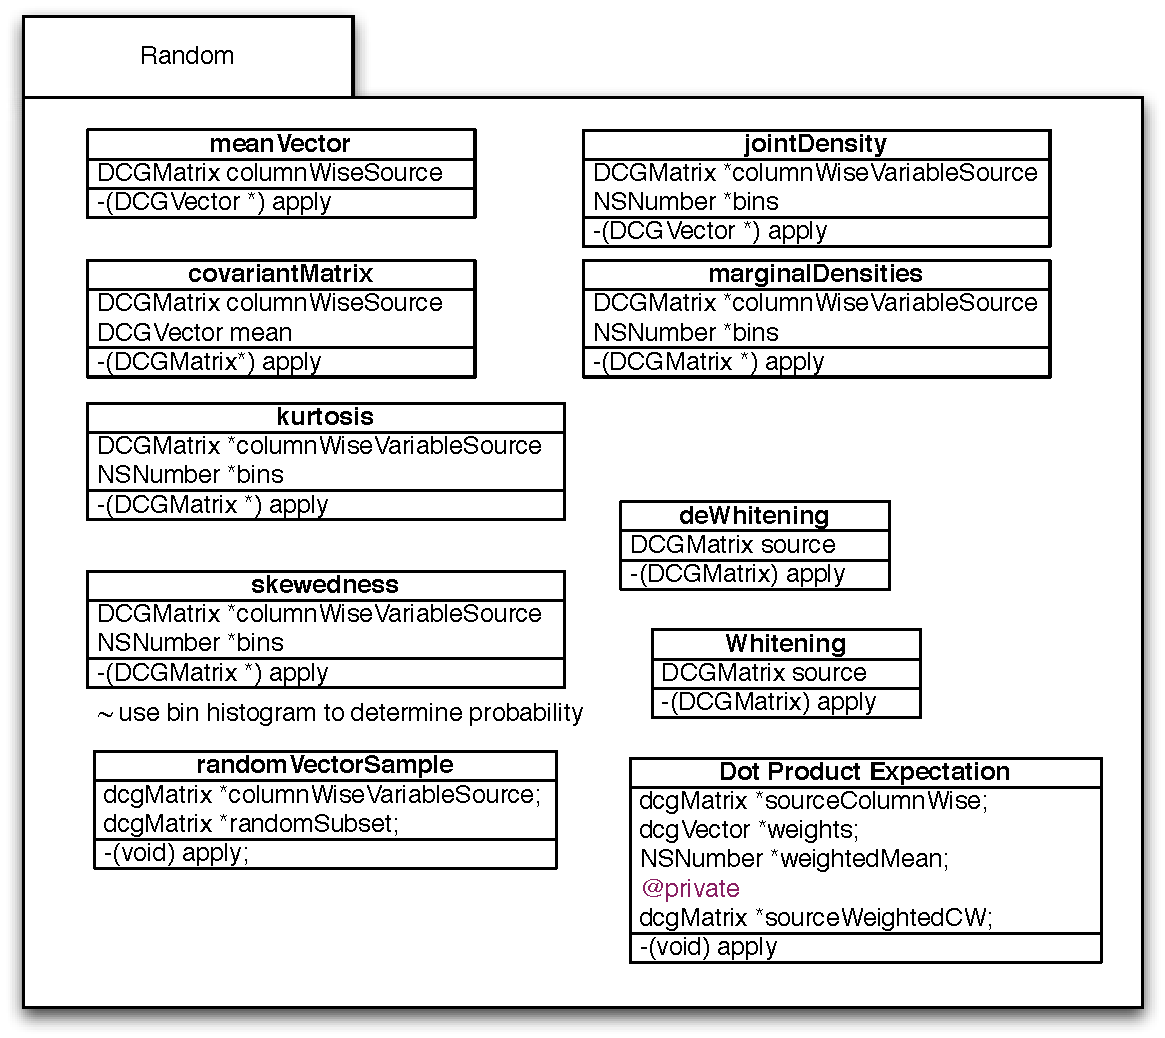
\includegraphics[width=4in]{randomFramework.pdf} 
   \caption{DCG Random Framework}
   \label{fig-random-framework}
\end{figure}

DCGRandom consists of property objects which correspond to general properties of random vectors.  These property objects are defined here.  %   
\begin{itemize}
\item Mean Vector
\begin{equation}
\vec{\mu} = E \{ \vec{x} \} 
\end{equation}

\item Covariance Matrix
\begin{equation}
\mathbf{ \Sigma} = E \{( \vec{x} - \vec{\mu})^2 \} 
\end{equation}
\item Skewness 
\begin{equation}
\mathbf{\Sigma} = E \{( \vec{x} - \vec{\mu})^3 \} 
\end{equation}
\item Kurtosis 
\begin{equation}
\mathbf{\Sigma} = E \{( \vec{x} )^4 \} - (E\{ \vec{x}^2 \} )^2 
\end{equation}
%\item Joint Density 
%\begin{equation}
%p(y_1, y_2, ..., y_n ) 
%\end{equation}
%As this applies to each of the observations a column vector of length satisfying the number of observations is needed to specify the probability of each observation.  In the case of continuous values, a naive classification of binning is used ( observation with in range).    In this case the bins are doubly naive as the binning applies to each column (attribute).  

%\item Marginal Densities
%\begin{equation}
%p(y_i  | y_1, y_2, ..., y_{i-1} , y_{i+1} , ..., y_n ) 
%\end{equation}
%Marginal densities simply apply to each variable and each observation.  The same binning scheme is applied in this case to observations, and histogram observations are then applied.   
\item Whitening 
\begin{equation}
A_w = \Lambda ^{-1/2} \Phi 
\end{equation}
where $\Lambda$ are the eigenvalues of the covariance matrix and $\Phi$ are the normalized eigenvectors.  
\item Dewhitening
\begin{equation}
A_w ^{-1}
\end{equation}
\end{itemize}
One point about the operational objects defined in this framework is how they are reused.  %The mean (univariate and multivariate) and variance (and covariance) show up in more complex objects in the DCG-Random framework.
Projection pursuit, the primary method of ICA used in this report, computes ICA by maximizing the average entropy.  Entropy is described in appendix \ref{entropy}

\section{ICA Family of Estimators}\label{mutual-independence}
The ICA family of estimators are unique regarding the items being estimated.   The standard ICA form is shown in equation \ref{standardICA}.  The dataset denoted by $\vec{x}$ is the only observed part.  The mixing matrix ($\mathbf{A}$,) the ICs ($\vec{s}$,) and the noise ($\vec{\nu}$) are all estimated.  If the noise can be assumed to be normal, then it can be eliminated from the standard ICA form to give the standard noiseless ICA form, equation \ref{standardICANoiseless}.  It is the inverse of the noiseless that allows for estimators of ICA to be constructed.
%\label{mutual-independence}
Standard form of ICA w/o noise
\begin{eqnarray}
\vec{x} = \mathbf{A}\vec{s} + \vec{nu} \label{standardICA} \\
\vec{x} = \mathbf{A}\vec{s} \label{standardICANoiseless} \\
\vec{s} = \mathbf{A}^{-1} \vec{x} \label{standardICAInverse} 
\end{eqnarray}

%Establish linear combinations that become the mixing matrix.  
Construction of an ICA estimator from equation \ref{standardICAInverse} requires a few algebraic manipulations.  These manipulations are show in equations \ref{unwhitenedICA} through \ref{whitenedICs}.
\begin{eqnarray}
y = \vec{b}^T \vec{x} \label{unwhitenedICA} \\
y = \vec{b}^T \mathbf{A}\vec{s} \\
\vec{q} = \mathbf{A}^{T} \vec{b} \\
y = \vec{q}^T \vec{s} \label{whitenedICs}
\end{eqnarray}
where
\begin{itemize}
\item $\mathbf{A}\vec{b}$ that maximizes $y$'s non-normal characteristics.
\item Such a $\vec{b}$ makes $\vec{q}$ have only one non-zero component.
\item Therefore, $y$ is an independent component.
\item Determining the non-normal characteristics has to contend with $\pm s_i$ as IC(s) can be determined up to a sign. 
\item This determination becomes an angle of sorts.  
\end{itemize}

One method for determining the non-normal characteristics is by kurtosis, shown in equation \ref{kurtosisStandardWhite}.  If $y$ is whitened source of data, then equation \ref{kurtosisStandardWhiteAssumed} holds.
%Non-Normal Character by Kurtosis
\begin{eqnarray}
\kappa _4 (y) = E \{ y^4 \} - 3 (E\{ y^2\})^2 \label{kurtosisStandardWhite}\\
E\{ y^2\} =1 \Rightarrow \kappa _4 (y) = E \{ y^4 \} - 3 \label{kurtosisStandardWhiteAssumed}%\\
%\kappa_4(y)  = m_4 (y)
\end{eqnarray}
The measure of Non-normal characteristics can be accomplished by $|\kappa_4(\dot)|$ and $\kappa_4 (\dot) ^2$.  %Note these properties:
Kurtosis has both additive and scaling properties as shown in equations \ref{addKurtosis} and \ref{scaleKurtosis}
\begin{eqnarray}
\kappa_4(x_1) + \kappa_4(x_2) \equiv k_4(x_1 + x_2) \label{addKurtosis}\\
\kappa_4(\alpha x) = \alpha \kappa_4 (x) \label{scaleKurtosis}
\end{eqnarray}

The objective is to apply kurtosis to $y$ (or its definition as an IC element).  Equation \ref{kurtosisAppliedToICACharacter} shows the application of kurtosis to the characteristic whitened equation of ICA.  A consequence of the data being whitened, shown in equation \ref{consequenceOfICACharacter}, is a reduction of terms for the characteristic equation.   From this consequence, the objective of finding each mixing vector translates to determining on the unit circle the maxima of $\kappa_4 (y)$.  In order to find the unit circle maxima, an assumption shown in equation \ref{icAssumptionUnitCircle}, the kurtosis of each IC is restricted to unit length.  
Therefore, gradient methods can be used to determine the kurtosis.
\begin{eqnarray}
\kappa_4(y) = \sum _i q_i \kappa_4 (s_i) \label{kurtosisAppliedToICACharacter}\\ 
E\{y^2 \} =1 \Rightarrow \sum_i q_i ^2 =1 \label{consequenceOfICACharacter} \\
\kappa_4(s_i) = 1 \Rightarrow F(\vec{q}) = \sum_i q_i ^4 \label{icAssumptionUnitCircle}
\end{eqnarray}

\subsection{Kurtosis Gradient Maximization}
Let $\vec{z}$ be $\vec{x}$ whitened and $\vec{w}$ be a whitened version of $\vec{b}$.  Then 
\begin{eqnarray}
y = \vec{w}^T \vec{z} \\ 
\kappa_4 (y) = \sum _i w_i \kappa_4{z_i} \\
\frac{\partial \kappa _4 (y)} {\partial \vec{w}} = 4 \textrm{sign} (\kappa _4 (y))E\{ \vec{z} (\vec{w}^T \vec{z})^3\} - 3 \frac{\vec{w}}{||\vec{w}||}  \\
\frac{\partial \kappa _4 (y)} {\partial \vec{w}} \approx 4 \textrm{sign} (\kappa_4(y))E \{ \vec{z} (\vec{w}^T \vec{z}) \} \\
\frac{\partial \kappa _4 (y)} {\partial \vec{w}} \to 0 
\end{eqnarray}
Thus if the partial derivative is set to zero, then the goal is to determine the roots which are the maxima and minima.  Note that $\vec{w}$ is to be normalized each iteration.  Note also the expectation operator in many cases is treated as a classic mean of the argument inside.    

%Note that if M = 1 and N > 1, then Projection Pursuit can only calculate X^T, not X itself. 
% Therefore $y = E (\vec{w}^T \vec{z}) = \vec{w}^T \vec{z}$, and $\Delta \vec{w} = E \{ y^3 \vec{z} \} = y^3 \vec{z}$.

% Supply algorithm here.

\begin{algorithm}
\caption{Projection Pursuit}
\label{alg:Projection-Pursuit}
\begin{algorithmic}
	\REQUIRE data source $\vec{x}$
	\REQUIRE Dot Product Expectation
	\REQUIRE Random Vector producer
	\STATE Center data to make its mean zero
	\STATE Whiten the data to provide $\vec{z}$
	\STATE $\vec{w} \leftarrow$ random vector
	\STATE Provide initial value for $\gamma$
	\REPEAT
		\STATE $y = E \{\vec{w}^T \mathbf{Z} \}$
		\STATE $ \Delta \vec{w} = E \{ \bar {y^3} \mathbf{Z}  \}   $
		\STATE $\vec{w} += \Delta \vec{w} $
		\STATE $\vec{w} \leftarrow \frac{\vec{w}}{||\vec{w}||}$
	\UNTIL {$\Delta \vec{w} \to 0$}
	\RETURN {$\vec{w}$}
\end{algorithmic}
\end{algorithm}



\subsection{Non-normality by Negentropy}
%\begin{equation}
%H(y) = - \int p_y (\nu) \log p_y (\nu)d\nu
%\end{equation}
One characteristic noted in 
\cite[94]{appo-ica-book} is that normal variables have the largest entropy of all random variables.  Appendix \ref{maximizing-via-negentropy} shows the theory of neg-entropy and its use in maximizing entropy. Two equations from the theory of neg-entropy, equations \ref{negentropyGauss} through \ref{normalEntropy}, can be used to approximate non-normality.  If $\vec{y}$ is used in these equations, then the fact that $\vec{y}$ is zero mean and unit variance (whitened) leads this estimation to the same estimation as kurtosis as shown equation \ref{whitenedNegentropyEstimation}.
%In this case, $y$ is a zero mean, unit variance random variable which may as well be whitened.  This is not good enough as it leads to the same issues as kurtosis.  
\begin{equation}
J(y) \approx k_1 ( E\{ G_1 (y)\} )^2 + k_2 [(E \{G_2 (y)\}) - (E \{G_2 (v)\}) ]^2 \label{whitenedNegentropyEstimation}
\end{equation}
This is why the entropy estimation via non-polynomial functions is considered.  %Suppose that 

\subsubsection{Negentropy Gradient Algorithm}
An non-polynomial approximation is shown in equation \ref{nonPolynomialApproximationNegentropy}.  Assuming that $G(\cdot)$ is defined as in $G_1$ or $G_2$, then applying constraints in equation \ref{normalConstraintOnMixer} through equation \ref{directionNegentropyNonPoly} lead to algorithms \ref{alg:FastICA-Stochastic-Negentropy-Projection-Pursuit} and \ref{alg:FastICA-Negentropy-Projection-Pursuit}.  Note that $v$ in these equations is a standardized normal variable.
\begin{eqnarray}
	J(y) \approx [(E \{G (y)\}) - (E \{G (v)\}) ] \label{nonPolynomialApproximationNegentropy} \\
G_1 (y) = \frac{1}{a_1} \log \cosh a_1 y \\
G_2 (y) = -\exp (\frac{-y^2}{2}) \\
E\{ (\vec{w}^T \vec{z} )^2 \} \to ||\vec{w}||^2 = 1 \label{normalConstraintOnMixer}\\ 
\Delta \vec{w} \propto \gamma E \{ \vec{z} (\vec{w}^T \vec{z}) \} \\
\vec{w} = \frac{\vec{w}}{||\vec{w}||}
\gamma = E \{G(\vec{w}^T \vec{z}) - E \{ G(v) \} \}  \label{directionNegentropyNonPoly}
\end{eqnarray}
%Again, $v$ is a standardized normal variable.
% 

\begin{algorithm}
\caption{FastICA Stochastic Negentropy Projection Pursuit}
\label{alg:FastICA-Stochastic-Negentropy-Projection-Pursuit}
\begin{algorithmic}
	\REQUIRE data source $\vec{x}$
	\STATE Center data to make its mean zero
	\STATE Whiten the data to provide $\vec{z}$
	\STATE $\vec{w} \leftarrow$ random vector
	\STATE Provide initial value for $\gamma$
	\REPEAT
		\STATE $\Delta \vec{w} \propto \vec{z}g(\vec{w}^T\vec{z})$
		\STATE $\vec{w} += \Delta \vec{w} $
		\STATE $\vec{w} \leftarrow \frac{\vec{w}}{||\vec{w}||}$
		\STATE $\Delta \gamma \propto (G(\vec{w}^T \vec{z}) E\{G(v)\}) - \gamma$
	\UNTIL {$\Delta \vec{w} \to 0$}
	\RETURN {$\mathbf{W}$}
\end{algorithmic}
\end{algorithm}


\begin{algorithm}
\caption{FastICA  Negentropy Projection Pursuit}
\label{alg:FastICA-Negentropy-Projection-Pursuit}
\begin{algorithmic}
	\REQUIRE data source $\vec{x}$
	\STATE Center data to make its mean zero
	\STATE Whiten the data to provide $\vec{z}$
	\STATE $\vec{w} \leftarrow$ random vector
	\REPEAT
		\STATE $\vec{w}_{old} \leftarrow \vec{w}$
		\STATE $\vec{w} \leftarrow E \{ \vec{z} g(\vec{w}^T \vec{z}) - E\{ g' (\vec{w}^T \vec{z}) \} \}$
		\STATE $\vec{w} \leftarrow \frac{\vec{w}}{||\vec{w}||}$
		\STATE $\Delta \vec{w} = \vec{w} - \vec{w}_{old}$
	\UNTIL {$\Delta \vec{w} \to 0$}
	\RETURN {$\mathbf{W}$}
\end{algorithmic}
\end{algorithm}

\subsection{Stability Analysis}
Each version of projection pursuit hinges on two theorems to guarantee convergence.  The solution of $J(y)$ is accomplished by an approximation of Newton's method to solve $J(\vec{w}^T \vec{z})$.
\begin{eqnarray}
	\vec{w} \leftarrow E \{ \vec{z} (\vec{w}^T \vec{z}) \} \\
	\approx E \{ \vec{z}g(\vec{w}^T \vec{z}) - E\{ g'(\vec{w}^T \vec{z}) \}\vec{w}^T \}
\end{eqnarray} 

\begin{quote}
	\begin{thm}
		Assume that the input data follows the ICA model with whitened data
			\begin{equation}
			\vec{z} = \mathbf{V A} \vec{s}
			\end{equation}
			where $\mathbf{V}$ is the whitening matrix, and that $G$ is a sufficiently smooth even function.  Then local maxima (resp. minima) of $E\{G(\vec{w}^T \vec{z}) \}$ under the constraint $||\vec{w}|| =1$ include those rows of the mixing matrix $\mathbf{V A}$ such that the corresponding independent components $s_i$ satisfy
			\begin{equation}
				E \{s_i g(\vec{s_i}) - g'(\vec{s_i}) \} > 0
			\end{equation}
			where $g(\dot) = G'(\dot)$, and $g'(\dot) = G''(\dot)$.
	\end{thm}
	\cite[187]{appo-ica-book}
\end{quote}
Therefore any nonquadratic can be used for $G(\dot)$.

\begin{quote}
	\begin{thm}
		Assume that the input data follows the ICA data model in (8.1), and that $G$ is a sufficiently smooth even function, then the asymptotically stable points of the algorithm in 
		\begin{eqnarray}
		\Delta \vec{w} \propto \gamma E\{ \vec{z}g(\vec{w}^T \vec{z}) \} \\
		\vec{w} = \frac{\vec{w}}{||\vec{w}||} 
		\end{eqnarray}
		include the ith row of the inverse of the whitened mixing matrix $\mathbf{V A}$ such that the corresponding independent components $s_i$ satisfies 
		\begin{eqnarray}
			g(\dot) = G'(\dot) \\
			E \{ s_i g(s_i) - g'(s_i) \} [ E \{ G(s_i) \} - E\{ G(v)\}] > 0
		\end{eqnarray}
		where $v$ is a standardized normal variable.
	\end{thm}
	\cite[187]{appo-ica-book}
\end{quote}

%The algorithm in question is called ``Fast Fixed-Point Non-Normality Maximization'' and is also known as FactICA Projection Pursuit via Negentropy.  
% Table 8.2 page 190

%\subsubsection{Multiple Independent Components}




\begin{algorithm}
\caption{FastICA Deflationary Orthogonalization}
\label{alg:FastICA-Deflationary-Orthogonalization}
\begin{algorithmic}
	\REQUIRE data source $\vec{x}$
	\REQUIRE number of ICs to estimate $m$
	\STATE Center data to make its mean zero
	\STATE Whiten the data to provide $\vec{z}$
	\FOR {p = 1 to M}
	\STATE $\vec{w_p} \leftarrow$ random vector
	\REPEAT
		\STATE $\vec{w_{old}} \leftarrow \vec{w_p}$
		\STATE $\vec{w_p} \leftarrow E \{ \vec{z} g(\vec{w_p}^T \vec{z}) - E\{ g' (\vec{w_p}^T \vec{z}) \} \}$
		\STATE Make orthogonal (GSO step) $\vec{w_p} \leftarrow \vec{w_p} - \sum _{j=1}{p-1} (\vec{w_p}^T\vec{w_j})\vec{w_j}$ 
		\STATE $\vec{w_p} \leftarrow \frac{\vec{w_p}}{||\vec{w_p}||}$
		\STATE $\Delta \vec{w_p} = \vec{w_p} - \vec{w_{old}}$
	\UNTIL {$\Delta \vec{w_p} \to 0$}
	\ENDFOR
	\RETURN {$\mathbf{W}$}
\end{algorithmic}
\end{algorithm}

\begin{algorithm}
\caption{FastICA Symmetric Orthogonalization}
\label{alg:FastICA-Symmetric-Orthogonalization}
\begin{algorithmic}
	\REQUIRE data source $\vec{x}$
	\REQUIRE number of ICs to estimate $m$
	\STATE Center data to make its mean zero
	\STATE Whiten the data to provide $\vec{z}$
	\FOR {p = 1 to M}
	\STATE $\vec{w_p} \leftarrow$ random vector
	\ENDFOR
	\REPEAT
	\STATE $\mathbf{W}_{old} = \mathbf{W}$
	
	\FORALL {$\vec{w_i} \in \mathbf{W}$ }
		\STATE $\vec{w_p} \leftarrow E \{ \vec{z} g(\vec{w_p}^T \vec{z}) - E\{ g' (\vec{w_p}^T \vec{z}) \} \}$
	\ENDFOR 
	\STATE Apply GSO to $\mathbf{W}$ 
	\STATE $\Delta \mathbf{W} = |\mathbf{W}_{old} - \mathbf{W}|$
	\UNTIL {$\Delta \mathbf{W} \to \mathbf{0}$}

	\RETURN {$\mathbf{W}$}
\end{algorithmic}
\end{algorithm}


\section{Sparse Coding Shrinkage}
Images also have characteristic equations, such as in equation \ref{image_character}.  The goal of Sparse Coding Shrinkage is to estimate $a_i$ and $s_i$ by forcing the spareness constraint.  %Thus to achieve this constraint the inverse of the characteristic equations is solved by optimizing $w_i$.
If the image values are treated as the $\vec{x}$ in ICA and $a_i$ and $s_i$ are their ICA equivalents, then ICA can estimate this characteristic equation. 

\begin{eqnarray}
%P \Rightarrow M \times N \\ 
I(x,y) = \sum _{i =1 }^n  a_i (x,y) s_i \label{image_character}%\\
%\mathbf{X} = \mathbf{A}\mathbf{S}
\end{eqnarray}


Sparse Coding Shrinkage represents basis vectors such that only a small number of basis vectors are activated at the same time.  \cite[397]{appo-ica-book}.  It is good for compression and de-noising.   In compression, sparse coding shrinkage endeavors to find the rare samples and allow them to be coded special from other more mundane samples.   In denoising, sparse coding shrinkage provides the independent components, and a selection of interest determines the ``really active'' components.  It is the de-noising part that the interest of this report. 

From all accounts of sparse coding shrinkage it is an application of ICA such that the local mean component is removed and the local variance is normalized.    Furthermore, PCA is applied to the data.   Sparse coding shrinkage does not specify that the procedure be restricted on how the data is arranged to obtain the mixing matrix.  

\cite[391-400]{appo-ica-book} used a neighborhood patch scheme, sampling $l \times l$ sections an arranging their values as one vector.  The complete set of samples compose the source matrix, and the mixing matrix with their independent components may be estimated.  Some experiments used a sliding neighborhood window as opposed to separating the matrix into patches. 

%One experiment not considered in \cite{appo-ica-book} was to use the features space of a multi-resolution wavelet transform.   Contrary to statements made by \cite{appo-ica-book}, the multiple resolutions of the wavelet transform need not use the same basis for each resolution.   As shown in the $\psi ^n$ resolution method, each resolution can treat each matrix an original matrix, and can reproduce the matrix based on the inverse wavelet transform for the same basis.   Thus any multi-basis-multi-resolution transform can identify any patch based on basis pair transformation and component of transformation. 

%Estimating ICA Basis from Image
%\begin{enumerate}
%	\item Remove the local mean component.  It is not certain to be sparse. 
%	\item Normalize local variance.
%	\item Combine the previous two steps by using PCA and dropping the least significant principal.
%	\item Use $l \times l$ patches (neighborhood size patches).
%\end{enumerate}
% Correct error on wavelet orientation.  

\subsection{Insert and Remove Noise on Patch Oriented Sparse Coding Shrinkage}


\begin{algorithm}
\caption{Insert and Remove Noise on Patch Oriented Sparse Coding Shrinkage}
\label{alg:patch-oriented-sparse-coding-shrinkage-with-source}
\begin{algorithmic}
	\REQUIRE Image source $I$
	\STATE Establish patches
	\STATE Insert a random sample patches column wise into data source $\mathbf{\mathcal{X}}_p$
	\STATE Estimate $\mathbf{\tilde{W}}$ for $\mathbf{\tilde{S}} = \mathbf{\tilde{W}}^T \mathbf{\mathcal{X}}_p$
	\STATE Insert noise
	\STATE Construct $\mathbf{\hat{S}}$ using $\mathbf{\tilde{W}}$ s.t. $\mathbf{\hat{S}} = \mathbf{\tilde{W}}^T \mathbf{\mathcal{X}}$
	\STATE Zero out whole columns of $\mathbf{\hat{S}}$ and construct $\mathbf{\hat{I}}$ with it. 
%	\RETURN {$\mathbf{W}$}
	\STATE Show $I$, noisy $I$ and $\mathbf{\hat{I}}$.
\end{algorithmic}
\end{algorithm}



\begin{algorithm}
\caption{Patch Oriented Source De-constructor}
\label{alg:Patch-Oriented-Source-Builder}
\begin{algorithmic}
	\REQUIRE Image source $I_m$
	\STATE $M$ is the number of rows in $I_m$
	\STATE $N$ is the number of columns in $I_m$
	\STATE $T$ is the total number of patches
	\STATE $M_p$ is the number of row patches. $M_p = \textrm{ceiling}(M / l)$
	\STATE $N_p$ is the number of column patches. $N_p = \textrm{ceiling}(N / l)$
	\STATE $T = M_p N_p$
	\FOR {each $\vec{h}_i \in \mathbf{H}$}
		\FOR {$x \in L(\vec{h}_i)$}
			\FOR {$y \in L(\vec{h}_i)$}
				\STATE $\vec{h}_i (x\% l +y) = I_m(x,y)$
			\ENDFOR
		\ENDFOR 
	\ENDFOR
	\RETURN $\mathbf{H}$
\end{algorithmic}
\end{algorithm}

\begin{algorithm}
\caption{Patch Oriented Source Builder}
\label{alg:Patch-Oriented-Source-Builder}
\begin{algorithmic}
	\REQUIRE Patch Oriented Source $\mathbf{H}$
	\FOR {$x_p \in M_p$}
		\FOR {$y_p \in N_p$}
			\STATE Insert $\vec{h_i}$ into $I(x,y)$
		\ENDFOR
	\ENDFOR
	\RETURN $\mathbf{I_m}$
\end{algorithmic}
\end{algorithm}

\begin{algorithm}
\caption{Patch Oriented Source Builder}
\label{alg:Patch-Oriented-Source-Builder}
\begin{algorithmic}
	\REQUIRE Image source $I$
	\STATE $M$ is the number of rows in I
	\STATE $N$ is the number of columns in I
	\STATE $T$ is the total number of patches
	\STATE $M_p$ is the number of row patches. $M_p = \textrm{ceiling}(M / l)$
	\STATE $N_p$ is the number of column patches. $N_p = \textrm{ceiling}(N / l)$
	\STATE $T = M_p N_p$
	\FOR {each $\vec{h}_i \in \mathbf{H}$}
		\FOR {$x \in L(\vec{h}_i)$}
			\FOR {$y \in L(\vec{h}_i)$}
				\STATE $\vec{h}_i (x\% l +y) = I(x,y)$
			\ENDFOR
		\ENDFOR 
	\ENDFOR
	\RETURN $\mathbf{X}$
\end{algorithmic}
\end{algorithm}

\begin{algorithm}
\caption{Insert and Remove Noise on Patch Oriented Sparse Coding Shrinkage}
\label{alg:patch-oriented-sparse-coding-shrinkage-with-source}
\begin{algorithmic}
	\REQUIRE Image source $I$
	\STATE Establish patches, $\mathbf{P}$
	\STATE Insert a random sample patches column wise into data source $\mathbf{\mathcal{X}}_p$
	\STATE Estimate $\mathbf{\tilde{W}}$ for $\mathbf{\tilde{S}} = \mathbf{\tilde{W}}^T \mathbf{\mathcal{X}}_p$
	\STATE Insert noise
	\STATE Construct $\mathbf{\hat{S}}$ using $\mathbf{\tilde{W}}$ s.t. $\mathbf{\hat{S}} = \mathbf{\tilde{W}}^T \mathbf{P}$
	\STATE Zero out whole rows of $\mathbf{\hat{S}}$ and construct $\mathbf{\hat{I}}$ with it. 
%	\RETURN {$\mathbf{W}$}
	\STATE Show $I$, noisy $I$ and $\mathbf{\hat{I}}$.
\end{algorithmic}
\end{algorithm}

These algorithm give rise to the need of a framework called patch world.  In actuality, patch world should consist of several smaller frameworks.. A patch framework is needed for neighborhoods, co-existing patches,  column-wise neighbors, and others not thought of at the time of this document.  
\begin{figure}[htbp] %  figure placement: here, top, bottom, or page
   \centering
   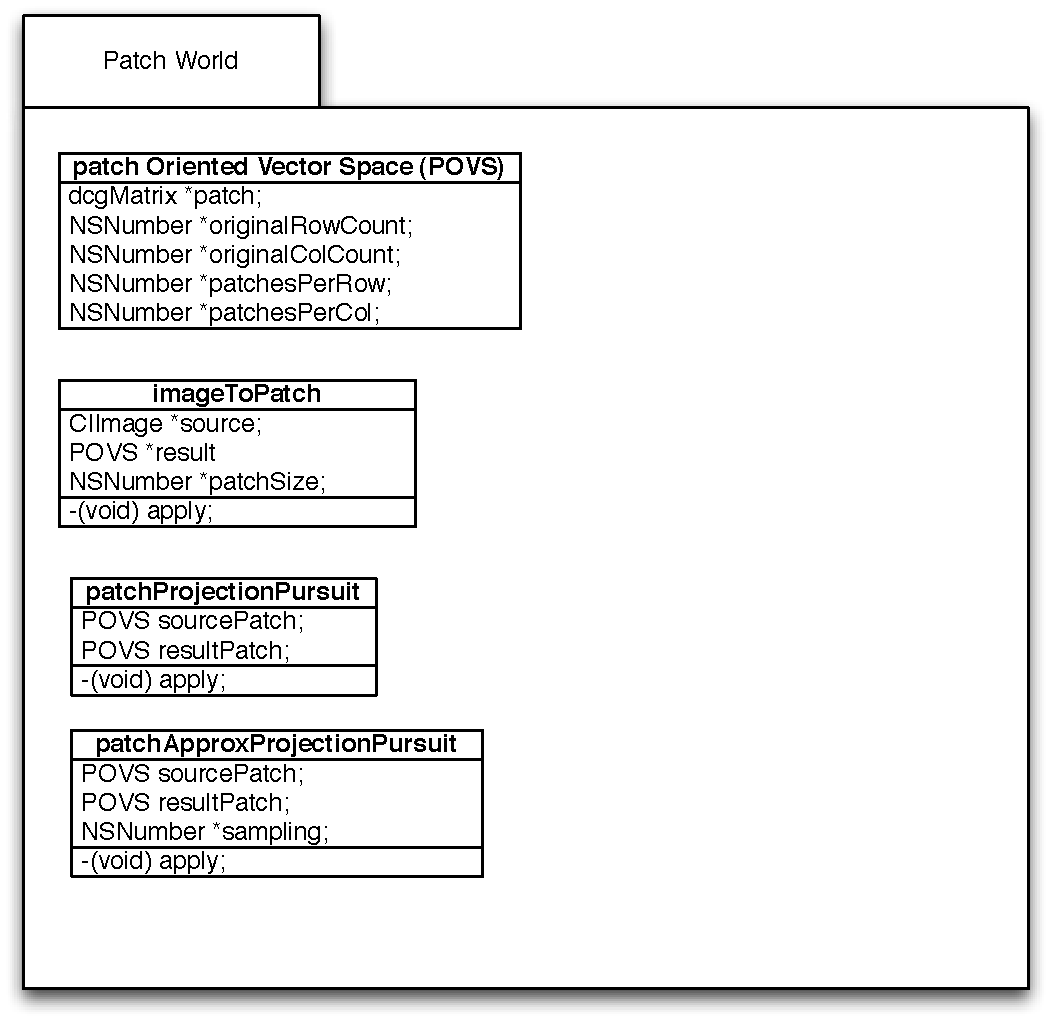
\includegraphics[width=4in]{patchWorld.pdf} 
   \caption{Patch World Framework}
   \label{fig-patch-world}
\end{figure}


\subsection{Connection between Independent Component Analysis and Sparse Code Shrinkage}
\label{ica-scs-connection}

The constraints on Sparse Code Shrinkage are included in the following list.  Accompanying these requirements are comments that show the connection to the objects of ICA. 
\begin{enumerate}
\item First, using a noise-free training set of $\vec{x}$, use some sparse coding method for determining the orthogonal matrix $\mathbf{W}$ so that the components $s_i$ in $\vec{s} = \mathbf{W}\vec{x}$ have as sparse distributions as possible.  Estimate a density model $p_i (s_i)$ for each sparse component, using the models in \ref{exponent} and \ref{Laplace}.
\begin{itemize}
	\item Note that if $\vec{x}$ is already whitened, then the ICA mixing matrix is a transformation matrix satisfying the constraints on $\mathbf{W}$.
	\item The exponential and Laplace density functions are specific components to the non-polynomial projection pursuit family. 
\end{itemize}


%\item Compute for each noisy observation $\mathbf{\tilde{x}}(t)$ of $\mathbf{x}$ the corresponding noisy sparse components $\mathbf{y}(t) = \mathbf{W}\mathbf{\tilde{x}}(t) $.  Apply the shrinkage non-linearity $g_i( \cdot)$ as defined in \ref{shrinkageGauss}, or in \ref{shrinkageLaplace}, on each component $y_i(t)$, for every observation index $t$.  Denote the obtained components by $\hat{s}_i (t) = g_i (y_i (t))$.
\item Invert the relation \ref{simpleICA} to obtain estimates of the noise-free $\mathbf{x}$, given by $\mathbf{\hat{x}}(t) = \mathbf{W}^T \hat{\mathbf{s}}(t)$.
\end{enumerate}
%This list can be a bit confusing as written, and needs a bit of explanation.  The value of $\vec{x}$ are the actual observed data set.  While there is no such thing as a noise free observed dataset, there is often an assumption that it is.  The reason is to simplify the fundamental equation of ICA from \ref{fundamental-ica} to \ref{fundamental-ica-noise-free}.
%\begin{eqnarray}
%	\vec{x} = \mathbf{A}\vec{s} + \vec{\nu} \label{fundamental-ica} \\
%	\vec{x} = \mathbf{A}\vec{s} \label{fundamental-ica-noise-free}
%\end{eqnarray}
The matrices $\mathbf{W}$ and $\mathbf{A}$ are mixing matrices.  Under the constraint that be both $\vec{s}$ and $\vec{x}$ are both zero mean and unit variant, $\mathbf{W}= \mathbf{A}^{-1} = \mathbf{A}^T$.


\section{Filters using ICA and PCA}\label{transformation-masking-maps}

\appendix
\section{Implementation of Projection Pursuit}

\begin{lstlisting} [ language={[Objective] C} ,caption={Projection Pursuit in Objective C}, label=lst_projectionPursuitApply ] 
-(void) apply
// Override on how the ICA algorithm is 
// computed.  Namely, this one is a 
// straight computation of projection 
// pursuit. 
{
[self prepareData];
int N = [samples colSize];
	
[randomAgent setLength:[NSNumber numberWithInt:N]];
[randomAgent apply];
dcgVector *w = [randomAgent randomVector];
dcgVector *wold;
dcgVector *deltaW;
double y;
Q = [NSNumber numberWithDouble:[w L2norm]];
do 
 {
  lastQ = Q;
  wold = w;
  y = [self dotProductExpectation:w];
  [meanVector setSourceColumnWise:
   [blasWork multiplyMatrix:whitenedData 
 	byScalar:pow(y, 3.0)]];
 	deltaW = [meanVector apply];

  w = [self addMixVector:w withDeltaVector:deltaW];
  Q = [NSNumber numberWithDouble:
		[blasWork dotProduct:w 
		byVector:wold]];
 }
 while (![self epsilonReached]);
}


\end{lstlisting}


\begin{lstlisting} [ language={[Objective] C} ,caption={Zero Mean Multivariate in Objective C}, label=lst_ZeroMeanMultivariate ] 
-(void) apply
{
 dcgBlasService *blasWork; 
 blasWork = [[dcgBlasService alloc] 
   init];
 dcgMatrix *workingMatrix;
 workingMatrix = [dcgMatrix zeroMatrix:
  [sourceColumnWise rowSize] 
  columns:[sourceColumnWise colSize]];
 int N = [sourceColumnWise colSize];
 int i;
 DCGMeanVector *meanVectorAgent;
 meanVectorAgent = [[DCGMeanVector alloc] init];
 [meanVectorAgent 
  setSourceColumnWise:sourceColumnWise];
 [self setMean:[meanVectorAgent apply]];
 for ( i = 0; i < N; i++)
 {
  [workingMatrix insertVector:mean atColumn:i];
 }
 [self setZeroMeanMultivariate:
   [blasWork subtractMatrix:sourceColumnWise 
   bMatrix:workingMatrix]];
 [blasWork release];
 [meanVectorAgent release];
}
\end{lstlisting}

\section{Theory of Estimators}
\begin{figure}[htbp] %  figure placement: here, top, bottom, or page
   \centering
   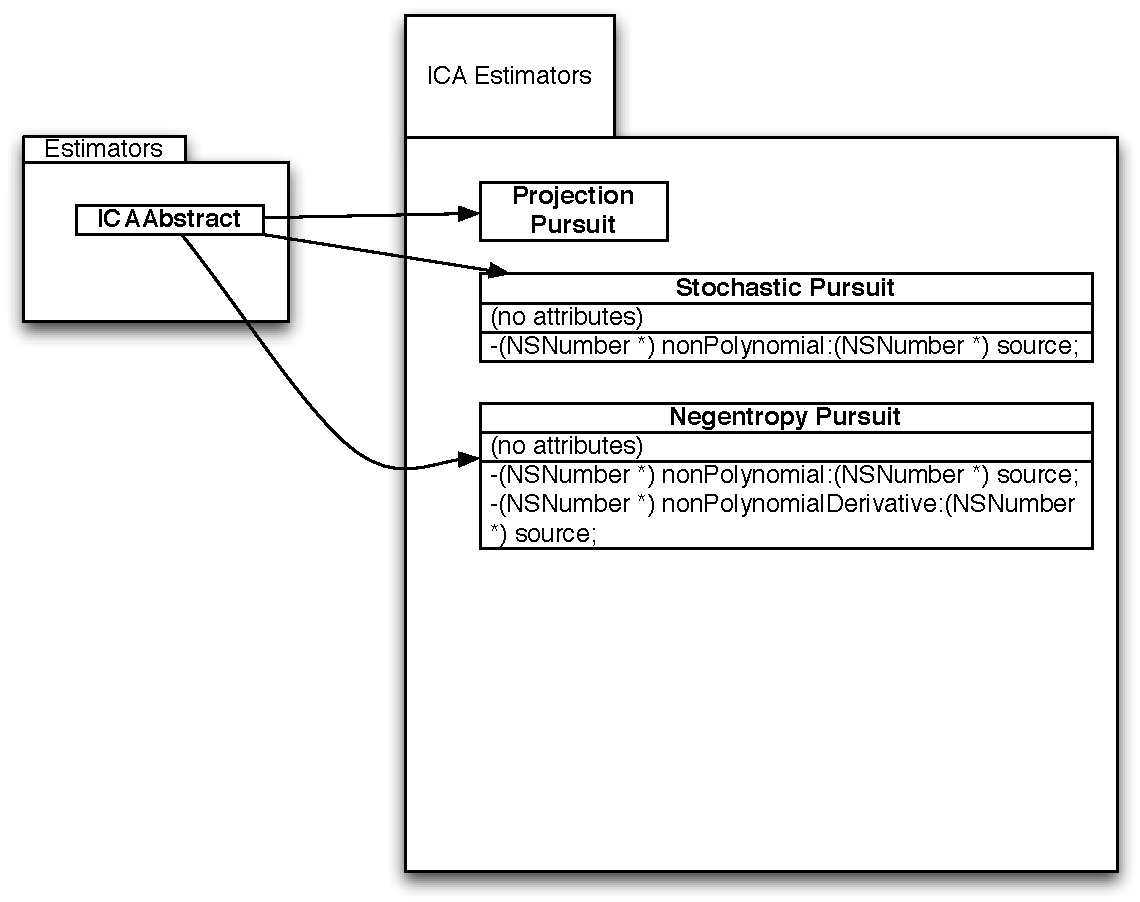
\includegraphics[width=4in]{estimators.pdf} 
   \caption{Estimators (ICA) Framework}
   \label{fig-estimator-world}
\end{figure}
%Unbiasedness and consistency
The theory of estimators is based on definition \ref{estimatorDefinition} and includes many linear and nonlinear methods to obtain the parameters thereof.   Estimators that achieve estimated parameters close to the actual parameters are called constant.  
%\begin{quote}
	\begin{adef}
		\label{estimatorDefinition}
	An estimator, $\hat{\mathbf{\theta}}$, of the parameter vector, $\vec{\theta}$, is the mathematical expression that estimates the parameters of an analytical solution for a given set of measurements (samples).
	\end{adef}

%\cite[78]{appo-ica-book}
%\end{quote}
There are a few constraints that any estimator should satisfy.   Estimators for which equations \ref{unbiasedEstimator} and \ref{unbiasedEstimatorGiven} are called unbiased.  
%Unbiased random parameters must satisfy one of the two equations: 
\begin{eqnarray}
E \{ \hat{\theta} \} \approx E \{\vec{\theta} \} \label{unbiasedEstimator}\\
E \{ \hat{\theta} | \vec{\theta} \} = \vec{\theta} \label{unbiasedEstimatorGiven}
\end{eqnarray}
Estimators not meeting this criteria are called biased.  The bias vector is defined 
\begin{eqnarray}
\vec{b} = E \{ \tilde {\theta} \} \\
\vec{b} = E \{ \tilde {\theta} | \vec{\theta} \} 
\end{eqnarray}
\begin{quote}
If $\vec{b} \to \vec{0}$ as the number of measurements goes up, then the estimator is called asymmetrically unbiased.
\cite[79]{appo-ica-book}
\end{quote}

Estimators often times require discrete items (called bins when forced on continuous values) in order to generate statistical models for datasets.  One important concept is the loss function as defined in Definition \ref{lossFunctionDefition}
\begin{quote}
\begin{adef}
	\label{lossFunctionDefition}
A loss function $h(\tilde{\theta})$ is a metric of the relative importance of specific estimation errors.
\end{adef}
\cite[79]{appo-ica-book}
\end{quote}
%Such loss functions include invariance of bins. 
Another important concept for estimators is their accuracy.  The article efficient is used as a ranking of an estimator as defined in Definition \ref{efficientEstimatorDefinition}.
%\begin{quote}
	\begin{adef}
		\label{efficientEstimatorDefinition}
An efficient estimator provides the smallest error covariance matrix among all unbiased estimators.	
	\end{adef}
\cite[81]{appo-ica-book}
%\end{quote}
Symmetry is also a means of ordering a matrix.  If $\mathbf{A}$ and $\mathbf{B}$ are both symmetrical matrices and $\mathbf{B} - \mathbf{A}$ is positive definite, then $\mathbf{A} < \mathbf{B}$.  One theorem, Cramer-Rao Lower Bound, provides for partial ordering amongst symmetric matrices.   This theorem is defined in theorem \ref{cramerRaoLowerBound}

%Crammer-Rao Lower Bound 
\begin{quote}
	\begin{thm}
	\label{cramerRaoLowerBound}
If $\hat{\theta}$ is any unbiased estimator of $\vec{\theta}$ based on the measurement data $\vec{x}$, then the covariance matrix of error in the estimator is bounded below by the inverse of the Fisher information matrix:
\begin{eqnarray}
J^{-1} \le E \{ (\vec{\theta} - \hat{\theta})(\vec{\theta} - \hat{\theta})^T | \vec{\theta} \} \\
J = E \{ [\frac {\partial} {\partial \vec{\theta}} \ln p(\vec{x_t} | \vec{\theta})] [\frac {\partial} {\partial \vec{\theta}} \ln p(\vec{x_t} | \vec{\theta})]^T | \vec{\theta} \}
\end{eqnarray}
	\end{thm}
\cite[83]{appo-ica-book}
\end{quote}

The last quality of an estimator considered is robustness.  Robustness is defined in Definition \ref{robustnessDefinition}.  Robustness determines an estimators ability accurately model a dataset despite the presence of outlier errors.  
\begin{quote}
	\begin{adef}
	\label{robustnessDefinition}
	Robustness is an insensitivity to gross measurement errors, and errors in specification of the parametric models.	
	\end{adef}
	\cite[83]{appo-ica-book}
\end{quote}

Both maximum-likelihood (ML) and expected maximization (EM) are covered in another report.  They may be reused in the pursuit of ICA, but in specific derivations thereof.  As this report does not cover the ML version of ICA, this report only eludes to it as an alternative estimator used to determine ICA. 



\subsection{Least Squares}
Least Squares regression is a linear method to determine specific parameters of an assumed analytical solution.  It is a classic curve fitting method which can be built to be solved by matrix solution methods like Gauss Jordan Elimination.
\begin{algorithm}
\caption{Least Squares Estimation (Regression) derived from definition found at \cite{wolfram-mathworld-least-squares}.}
\label{alg:least-squares}
\begin{algorithmic}
\REQUIRE DCGVector $\vec{x}$ consisting of $m$ observations
\REQUIRE Assumed model, parameters, and derived functions.
\STATE Take an initial guess at the model parameters $\lambda _i$ $\forall _i \in [1, n]$.
\REPEAT
\STATE Form matrix $A$ such that 
\begin{equation}
\left(\begin{array}{ccc}
	\frac{\partial {f(x)} } {\partial{\lambda_1}} |x_1 & ... & \frac{\partial {f(x)} } {\partial{\lambda_n }} |x_1 \\
	... & ... & ... \\
	 \frac{\partial {f(x)} } {\partial{\lambda_1}} |x_m & ... &  \frac{\partial {f(x)} } {\partial{\lambda_n}} |x_m
\end{array}\right)
\end{equation}
\STATE Compute $R = A^T A$ 
\STATE Compute $dB$ such that 
\begin{equation}
B = \sum _{i= 1} ^{m} ( y_i - f(x) )
\end{equation} 
\STATE Determine $L = A^T dB$
\STATE Determine $\partial \vec{\lambda}$ from $R(\partial {\vec{\lambda}}) = L $
\STATE Adjust $\vec{\lambda}$ by $\partial \vec{\lambda}$
\UNTIL {$d\vec{\lambda} \to 0$ }
\end{algorithmic}
\end{algorithm} 
From this algorithm, there are a family of least squares estimators.   Each one with their own assumed model and parameters.   There is a general class for polynomials.   Other models such as Gaussian or other statistical models should be developed with rules stated above for the univariate cases. 

	\begin{itemize}
	\item The desired property is to have more measurements than parameters (known or unknown)
	\item The goal is to choose an estimator that minimizes the effects of the error.
	\end{itemize}




\subsection{Maximum a Posteriori} 
Maximum a Posteriori is based on Bayes Theorem, theorem \ref{bayesTheorem}.  The characteristic equation for a given set of data is the sum of a set of distributions.   Each parameter of this characteristic equation can be determined by least squares regression.  This principal comes from the Optimal Estimator Theorem.  

\begin{eqnarray}
p_{\vec{\theta} | \vec{x_t}}(\vec{\theta} | \vec{x_t}) = \frac{p_{\vec{x_T} | \vec{\theta}}(\vec{x_T} | \vec{\theta}) p_{\vec{\theta}} (\vec{\theta})} { p_{\vec{x_T}} (x_T)  } \label{bayesTheorem}\\
p_{\vec{x_T}} (x_T)  = \int _{-\infty} ^{\infty} p_{\vec{x_T} | \vec{\theta}}(\vec{x_T} | \vec{\theta}) p_{\vec{\theta}} (\vec{\theta}) d\vec{\theta}
\end{eqnarray}


\begin{quote}
\begin{thm}
	\textbf{Optimal Estimator Theorem:} Assume that the parameters $\vec{\theta}$ and the observations $\vec{x_T}$ have the joint probability density function $p_{\vec{\theta} , \vec{x_t}}(\vec{\theta} , \vec{x_t})$.  The minimum mean-square estimator $\hat{\theta}_{MSE}$ of $\vec{\theta}$ is given by the conditional expectation:
\begin{equation}
\hat{\theta}_{MSE} = E[\vec{\theta} \vec{x_T}]
\end{equation}
\end{thm}
\cite[94]{appo-ica-book}
\end{quote}

The goal of Maximum a Posteriori to find the parameter vector $\vec{\theta}$ that maximizes the posterior density of the Bayes Theorem equation. The parameters are also based on an analytically defined model.  In this case, the $\vec{\theta}$ needs to maximize the numerator, as the denominator does not depend on $\vec{\theta}$.
\begin{eqnarray}
p_{\vec{\theta} | \vec{x_t}}(\vec{\theta} | \vec{x_t}) \approx p_{\vec{x_T} | \vec{\theta}}(\vec{x_T} | \vec{\theta}) p_{\vec{\theta}} (\vec{\theta}) d\vec{\theta} \\
\ln p_{\vec{\theta} | \vec{x_t}}(\vec{\theta} | \vec{x_t}) \approx \ln (p_{\vec{x_T} | \vec{\theta}}(\vec{x_T} | \vec{\theta}) p_{\vec{\theta}} (\vec{\theta}) d\vec{\theta}) \\
 \approx \ln( p_{\vec{x_T} | \vec{\theta}}(\vec{x_T} | \vec{\theta})) + \ln (p_{\vec{\theta}} (\vec{\theta}) d\vec{\theta} )\\
%\frac{\partial} {\partial \vec{\theta} } \ln p_{\vec{\theta} | \vec{x_t}}(\vec{\theta} | \vec{x_t}) \\ 
\approx 
\frac{\partial} {\partial \vec{\theta} } \ln( p_{\vec{x_T} | \vec{\theta}}(\vec{x_T} | \vec{\theta})) + \frac{\partial} {\partial \vec{\theta} } \ln (p_{\vec{\theta}} (\vec{\theta}) d\vec{\theta} ) \label{ln_bayes}
\end{eqnarray}


Given these equation the solution can be defined by setting equation \ref{ln_bayes} to zero.
\begin{equation}
 \frac{\partial} {\partial \vec{\theta} } \ln( p_{\vec{x_T} | \vec{\theta}}(\vec{x_T} | \vec{\theta})) + \frac{\partial} {\partial \vec{\theta} } \ln (p_{\vec{\theta}} (\vec{\theta}) d\vec{\theta} ) = 0 
\end{equation}

Like ML and EM, MAP is mentioned here as an alternative means of determining ICA.   MAP itself does not provide ICs.  Rather it provides an intermediate step from which ICA may be determined.   

\section{Entropy and Mutual Information: Determining Independence}\label{entropy}
One of the most crucial features of the ICA estimator is the ability determine independence.  Two fundamental concepts that lead to deterministic methods of independence are entropy and mutual information.  As these two concepts are very much related, they are presented in this sub-section.

\subsection{Measures of Information}
%\subsubsection{Differential Entropy}
The concept of entropy is best stated in its differential form, both discrete and continuous.  Entropy can be treated as a measure of the amount of information contained in a specific data set.  In the discrete case, this concept can determine encoding necessary to represent the data.
\begin{eqnarray}
H(X) = \sum_i f(P(X =a_i)) \\
H(x) = - \int p_x (\eta) \log p_x (\eta) d\eta = \int f(p_x(\eta))d\eta
\end{eqnarray}
Note that transforming entropy increases/decrease monotonically.  %It causes scalar multiplication of values to increase entropy by the same logarithmic scalar.

%\subsubsection{Mutual Information}
The metric of mutual information between scalar random variables, a measure of information that one random variable has on the other random variables in a set, is defined in terms of a single random variable $x_i$  
\begin{equation}
I(\mathbf{X},\mathbf{Y})  = H(\mathbf{Y}) - H(\mathbf{Y}|\mathbf{X}) = H(\mathbf{X}) - H(\mathbf{X}|\mathbf{Y})
\end{equation}
\begin{quote}
Maximizing the joint entropy $H(Y_1, Y_2)$ is accomplished by maximizing the individual entropies while minimizing the mutual information $I(Y_1, Y_2)$.  When $I(Y_1, Y_2)$ is zero, then $Y_1$ and $Y_2$ are statistically independent.
\cite[662]{moon-stirling-book}
\end{quote}

%Neither entropy nor mutual information can be treated as a metric as there is not applicable inversion from the measure to the data.  

%\subsubsection{Kullback-Leibler Divergence}
The purpose of Kullback-Leibler Divergence is provide a pseudo metric in terms of distance  between two density functions, and therefore determine mutual information.   It is not a true metric since it is not symmetric.   Yet, the Kuller-Leibler Divergence does increase monotonically with mutual information.  

\begin{eqnarray}
\Delta(p| q) = \sum _i p(i) (\log p(i) - \log q(i)) \\
\Delta(p| q) = \int p(i) (\log p(i) - \log q(i)) 
\end{eqnarray}


\subsection{Theory of Maximizing Representation}\label{maximizing-represnetation}

%\subsubsection{Maximum Entropy}
The goal of maximum-entropy is to determine the probability density function that satisfies equation \ref{constant-entropy} such that the $c_i$ constants are maximum.  One example under some regularity conditions is equation \ref{regularity-condition-constraint-for-entropy} (under the constraint in equation \ref{regularity-condition-constraint-for-entropy}.
\begin{eqnarray}
\int p(\eta) F_i (\eta) d\eta =  c_i \label{constant-entropy} \\
p_0( \eta) = A \exp (\sum_i a_i F_i (\eta)) \label{regularity-condition-constraint-for-entropy} \\
\int p_0 (\eta) d \eta = 1 \label{system-regularity-condition-constraint-for-entropy} 
\end{eqnarray}


\subsubsection{Negentropy}\label{maximizing-via-negentropy}
Negentropy is a concept derived from maximum entropy specifically for determining Gaussian properties.  The objective is to have ``a measure that is zero for a Gaussian variable and always nonnegative can be simply obtained from differential entropy.''  Negentropy, denoted $J(\vec{x})$, is defined in equation \ref{negentropy}.  The entropy of $x_{Gauss}$ is defined in terms the covariance matrix of $\vec{x}$ ($\Sigma$) and the dimension of $\vec{x}$.
\begin{eqnarray}
J(\vec{x}) = H(\vec{x}_{\textsl{Gauss}}) - H(\vec{x}) \label{negentropyGauss}\\
H(\vec{x}_{\textsl{Gauss}}) = \frac{1}{2}\log |\det \Sigma | + \frac{n}{2}[1 + \log {2\pi}] \label{normalEntropy}
\end{eqnarray}
Properties of negentropy include:
\begin{itemize}
	\item $J(\vec{x}) = 0$ i.f.f. $\vec{x}$ has a Gaussian distribution.
	\item The maximum Gaussian distribution satisfying equation \ref{constant-entropy} forces $J(\vec{x}) \ge 0$
	\item invariant to invertible linear transformation as proven in \cite[113]{appo-ica-book}.
\end{itemize}



\subsubsection{Approximation by Cummulants}
Polynomial density expansion approximation of negentropy, maximum entropy, and mutual information is defined for a standardized Gaussian model (zero mean and unit variance) as in equation \ref{standardized-Gaussian}, and its derivative in equation \ref{standardized-Gaussian-first-derivative}.  The polynomial system is chosen for the practicality that they are orthogonal.  
\begin{eqnarray}
\phi (\eta) = \frac{1}{2\pi} \exp (\frac{-\eta}{2}) \label{standardized-Gaussian}
\frac{\partial ^i \phi (\eta)} {\partial \eta} = (-1)^i H_i(\eta)\phi (\eta) \label{standardized-Gaussian-first-derivative}
\end{eqnarray}

Another approximation that maximize representation is the log of the cumulants.  This approximation depends on the cumulants being relatively small.  
\begin{equation}
\log (1 + \epsilon) \approx \epsilon - \frac{\epsilon ^2}{2}
\end{equation}
%The non-Gaussian portions of the polynomial density expansion are part of the skewness and kurtosis.  Thus a class by the name of kurtosisApproxNegentropy.  This approximation is derived from the definition of entropy:
Therefore, cumulants can be used to define a characteristic equation for the information carried in a dataset $x$.
\begin{eqnarray}
	p_x(\eta) \approx \phi (\eta)(1 + \kappa_3 (x) \frac{H_3(\eta)} {3!}+ \kappa_4 (x) \frac{H_4(\eta)} {4!}) \\
%H(x) = - \int p_x (\eta) \log p_x (\eta) d\eta = \int f(p_x(\eta))d\eta \\
%H(x) \approx - \int \phi (\eta)(1 + \kappa_3 (x) \frac{H_3(\eta)} {3!}+ \kappa_4 (x) \frac{H_4(\eta)} {4!}) \frac{1}{2}[\log (\phi (\eta)(1 + \kappa_3 (x) \frac{H_3(\eta)} {3!}+ \kappa_4 (x) \frac{H_4(\eta)} {4!}))] \\
%H(x) \approx - \int \phi (\eta)(1 + \kappa_3 (x) \frac{H_3(\eta)} {3!}+ \kappa_4 (x) \frac{H_4(\eta)} {4!}) \frac{1}{2}[\log \phi (\eta) + \log \phi(\eta) \kappa_3 (x) \frac{H_3(\eta)} {3!}+ \log \phi(\eta)\kappa_4 (x) \frac{H_4(\eta)} {4!}]\\
%H(x) \approx - \int \phi (\eta)(1 + \kappa_3 (x) \frac{H_3(\eta)} {3!}+ \kappa_4 (x) \frac{H_4(\eta)} {4!}) \frac{1}{2}[\log \phi (\eta) +  \kappa_3 (x) \frac{H_3(\eta)} {3!}+  \kappa_4 (x) \frac{H_4(\eta)} {4!} ( \kappa_3 (x) \frac{H_3(\eta)} {3!}+  \kappa_4 (x) \frac{H_4(\eta)} {4!})^2] \\
J(x) \approx \frac{1}{12} \kappa_3 (x) ^2 + \frac{1}{48} \kappa_4 (x) ^2
\end{eqnarray}
Thus a sum of the skewness squared and the kurtosis squared (both computable from the random framework.)  The drawback is that this method is sensitive to outliers and it measures the tails and not the center.   It is thus worth considering methods of determining entropy by non-polynomial functions.   The constraints on such methods are as follows:
%\subsubsection{Approximation of Entropy by Non-Polynomial Functions}
\begin{itemize}
\item Based on maximum entropy methods
%\item Bypasses the finite expectation functions and approximations there of.  
\item Confines the distribution from the infinite  which will satisfy to a specific set of constraints.  
%\item Called the maximum entropy method, it is a ``first order approximation'' for a continuous one-dimensional random variable.  
\end{itemize}
These constraints allow for a first order approximation to be constructed for a one-dimensional random variable.  GSO also for multiple-dimensional random variables to approximated by applying this process to each variable, and orthogonalizing the variables at the end of each iteration.  An example for determining non-polynomial functions that achieve this are Gram-Charlier as shown in equation  \ref{general-nonpolynomial}.

%\begin{enumerate}
%\item Estimate expectations on $\vec{x}$
%\item $E(G_i (x))$ is not statistically difficult to estimate.  Thus no functions that grow faster than quadratics.  Log-densities on the other hand may be suitable.
%\item Is not sensitive to outliers (typically).
%\item $p_0$ is assumed to be integratable.
%\item The $G_i(x)$ must capture aspects of the distribution of $X$ that are pertinent in the computational entropy.  
%\end{enumerate}

%In these examples, Gram-Charlier becomes a useful tool for determining the coefficients.  The general form of this negentropy approximation is defined in equation \ref{general-nonpolynomial}.
\begin{equation}
J(x) \approx k_1 (E\{G_1 (x) \}  )^2  k_2 (E \{G_2(x) \} - E\{G_2 (\mathcal{V}) \})^2 \label{general-nonpolynomial}
\end{equation}

% Note this portion represents difficulty in understanding.  It is difficult to determine where the math is going in this case.  



\bibliography{../patternNotes.bib}
\bibliographystyle{abbrv}
\end{document}
